
%
% ---- Chapter layout ----
%
% 1) Introduction - 
% 2) 
% ------------------------



\chapter{Biogenic Isoprene emissions in Australia} % Chapter title
\label{BioIsop}
  
%----------------------------------------------------------------------------------------
% Section 1 -- INTRO 
%----------------------------------------------------------------------------------------
\section{Introduction}  
\label{BioIsop:intro}  
  
  
  
  % isoprene and Australia
  Isoprene has a large impact on the oxidative properties of the atmosphere, as it reacts quickly with the OH radical to form RO$_2$.
  These react quickly with NO$_X$ to form OVOCs (such as HCHO), SOAs, and ozone.
  Australian isoprene emissions are poorly understood due to poor measurement coverage, and poor emission factor characterisation.
  The emissions of isoprene have been modelled at around 500\tgcpyr in \textcite{Guenther1995,Guenther2006} using MEGAN, and more recently around 465\tgcpyr in \textcite{Messina2016} using ORCHIDEE.
  The global emission models used to derive these estimates are based on modelling emissions from different plant species (phenotypes), of which few are used when setting the emission factors of Australian forests.
  Satellite based emissions estimates may allow us to improve the models without requiring other expensive measurements over the large data sparse continent of Australia.
  
  Modelled isoprene and BVOC emissions from MEGAN \parencite{Guenther2000} of 500 and 1150~Tga$^{-1}$ respectively are still the global go-to estimates.
  BVOC emissions are rising globally, and improved estimates for Australia is a priority due to their high uncertainty.
  \textcite{Kefauver2014} reviews remote sensing of BVOC emissions, examining the last 20 years of data and analysis of the satellite products.
  Their review reinforces the message that NMVOCs affect the oxidative capacity of the atmosphere and are largely driven by and sensitive to vegetation.
  The tropospheric effects of NMVOCs on the hydroxyl radical (OH), ozone (O$_3$), SOAs, and methane longevity all interconnect to form a very complex system which still suffers from relatively large uncertainties in both measurement and chemistry mechanisms.
  
  In this chapter the top-down technique using satellite measurements of HCHO to estimate surface isoprene emissions is used.
  Direct isoprene measurements are costly and sparse within Australia, and satellite measurements are plentiful and freely available, making this technique very attractive.
  Such techniques have informed isoprene emission inventories in North America \parencite{Abbot2003,Palmer2003,Palmer2006,Millet2006,Millet2008}, South America \parencite{Barkley2013}, Europe \parencite{Dufour2009,Curci2010}, Africa \parencite{Marais2012}, Asia \parencite{Fu2007,Stavrakou2014}, India \parencite{Surl2018}, and even globally \parencite{Shim2005,FortemsCheiney2012,Bauwens2016}.
  HCHO is the dominant product of most BVOCs and is measured by remote sensing.
  The main datasets of HCHO are from four satellite instruments: GOME on ERS-2, SCIAMACHY on ENVI-SAT, OMI on EOS AURA, and GOME2 on MetOp-A.
  These satellites have slightly different spectral and spatial resolutions, as well as using varied processes to estimate HCHO from detected radiances.
  This can lead to different estimates between instruments or methodologies as described in \textcite{Lorente2017}, which means validation and comparison is more important when using these remotely sensed data.
  In this thesis the dataset from the OMI instrument (\ref{Model:Datasets:Aura}) is used as the basis for HCHO amounts.
  
  \subsection{Aims}
    
    %% AIMs paragraph
    Recently isoprene measurements have suggested that modelled emissions may be overestimated in southeastern Australia, while
    emissions of monoterpenes (C$_{10}$H$_{16}$, two units of isoprene) appear to be underestimated \parencite{Emmerson2016}. 
    This could lead to the unique scenario of neither emission type dominating VOC chemistry over the forests.
    This work aims to improve isoprene emission estimates in Australia, which remain relatively uncertain.
    Here we introduce how uncertain isoprene emissions are over Australia, and discuss literature which shows how the estimates may be too high.
    We also describe how emissions may be calculated using satellite datasets.
    Additionally we outline why current isoprene emissions estimates are inadequate and how they can be improved.
    Section \ref{BioIsop:Methods} lays out how new isoprene emissions are estimated, and results are examined in Section \ref{BioIsop:Results}. 
    In section \ref{BioIsop:Affects} we examine how these changes in emissions would affect ozone concentrations in Australia, along with some other chemical processes.
    Uncertainties for each step along the way are quantified in section \ref{BioIsop:Uncertainty}.
  
    % What we aim to do
    We estimate isoprene emissions in Australia using top-down estimates based on OMI HCHO measurements and modelled isoprene to HCHO yields.
    The OMI HCHO total columns are recalculated using an updated estimate of HCHO profiles from GEOS-Chem v10.01 (see chapter \ref{Model}).
    These estimates are compared to several campaigns (SPS1, SPS2, MUMBA, Daintree) 
    Sensitivity to soil moisture, (maybe) LAI, and satellite AMF calculation is examined and quantified for some scenarios.
    The effect of using these new top down isoprene emissions as the boundary conditions for GEOS-Chem is studied
    Wellness of fit between in-situ (at Wollongong) HCHO, satellite (OMI), and modelled (GEOS-Chem) HCHO is determined with and without updated emissions estimates.
    
  \subsection{MEGAN emission model}
    % Megan estimates BVOCs - uncertain
    The Model of Emissions of Gases and Aerosols from Nature (MEGAN) is one of the most popular emissions inventories for biogenic isoprene.
    Global atmospheric studies often use MEGAN along with a chemical transport model (CTM) to examine transport, emission, deposition, and other chemical processes in the atmosphere.
    Emissions of Biogenic Volatile Organic Compounds (BVOCs) including isoprene are often the subject of studies as they are still relatively uncertain, as well as being drivers for important oxidation and pollution events.
    
    (MEGAN) is poorly calibrated for Australian conditions, and emissions of isoprene (C$_5$H$_8$) may be overestimated, especially in the southeast.
    \textcite{Stavrakou2015} showed that this overestimate may be a factor of 2-3 in January.
    \textcite{Sindelarova2014} show how 50\% of the isoprene emissions could be reduced by accounting for lower soil moisture.
    \textcite{Emmerson2016} discuss the suitability of MEGAN's isoprene and monoterpene emission factors over southeast Australia, and suggest isoprene emissions are estimated 2-6 times too high.
    They also show that no blanket increase or decrease in emission factors is appropriate for the entire southeast of Australia.
    This work tries to improve the understanding of isoprene emissions in Australia, clarifying the spatial distribution of bias and how these biases impact modelled chemistry.
  
  \subsection{satellite inversions}
    \label{BioIsop:intro:satellite_inversion}
    % Lead in to satellite inversion
    Top-down estimates look at how much of a chemical is in the atmosphere and try to work out how much of its major precursors were emitted.
    This generally takes advantage of longer lived products which may reach a measurable equilibrium in the atmosphere.
    For isoprene this is done by looking at atmospheric HCHO enhancement, which can be largely attributed to isoprene emissions once transport and other factors are accounted for.
    %Even anthropogenic HCHO source estimates, which are accurate at the global scale, can be improved using satellite data to improve regional estimates by up to 25-40\% \parencite{Stavrakou2015}. 
    %Their study used the RETRO 2000 database for anthropogenic emission aprioris except for Asia in 2008 where REASv2 was used. 
    Since 1997, when GOME first measured HCHO over Asia \parencite{Thomas1998}, satellites have been able to provide a total column measurement of HCHO, allowing isoprene emissions estimates by proxy \parencite{Palmer2001,Bauwens2016}.
    Using satellite information to improve biogenic emissions is pinpointed as a valuable use of satellite derived datasets \parencite{Streets2013}.
    In this work we use NASA's OMHCHO product, using measurements from OMI on board the AURA satellite (see section \ref{Model:Datasets:Aura}).
    
    % Brief isoprene to hcho description
    In the remote troposphere HCHO production is dominated by methane oxidation, while in the continental boundary layer (CBL) production is largely due to NMVOCs \parencite{Abbot2003, Kefauver2014}.
    This suggests that HCHO enhancement over continents can be used to determine NMVOC emissions.
    In the CBL, HCHO enhancement is generally driven by short lived ($<1$~hr) precursors (most importantly isoprene).
    HCHO itself has a lifetime of a few hours \parencite{Kefauver2014}.
    Isoprene is emitted and enters the atmosphere in the gas phase, where it begins a complex series of reactions.
    Formaldehyde is produced with high yields in many of the isoprene reactions, which are discussed in more detail in Section \ref{LR:VOCs:IsopCascade}.
    HCHO measurements are often used as a check on how well isoprene reactions are simulated, as model output can then be compared against them \parencite{Marvin2017}.
    
    Satellites recording reflected solar spectra use DOAS to measure various trace gases in the atmosphere, including formaldehyde. 
    While satellite measurements can only be used during daytime hours, HCHO lifetimes are sufficiently short that any night-time chemistry will not affect midday observations \parencite{Wolfe2016}.
    Satellites can be used to measure the seasonal and inter annual variability of HCHO over the globe.
    These records can be compared with modelled estimates of HCHO and also used as a proxy to estimate isoprene emissions.
    Total HCHO is measured by satellite over the entire world, however the technique is not perfect and suffers from uncertainties.
    Satellite based chemical concentrations often require both remote and in-situ measurements combined with modelled data for validation \parencite{Marais2014}.
    There is less information available from satellite measurements at higher latitudes due to increased error in measurements over the more slanted column paths \parencite{DeSmedt2015}.
    
    
    Validation is important due to the various uncertainties in the satellite remote sensing process, with apriori assumptions having the greatest effect on structural uncertainty between measurements techniques \textcite{Lorente2017}.
    \textcite{Zhu2016} use SEAC$^4$RS aircraft HCHO measurements over the southeastern US as model validation, and show a bias in the assumed OMI shape factor that leads to a bias between satellite and SEAC$^4$RS measurements.
    \textcite{Marais2014} compare OMI based isoprene emission estimates against relaxed eddy accumulation measurements from African field campaigns in order to improve MEGAN emission factors in the region.
    \textcite{Dufour2009} use HCHO from SCIAMACHY, and examine Europe using CHIMERE as the chemical model, showing that satellite measurements can reduce source emission uncertainty by a factor of two, where emissions are relatively large.
    
  
  \subsection{Top-down emissions estimates}
    
    % First isoprene inversion work
    We broadly follow the method of \textcite{Palmer2001} to create an emissions estimate of isoprene over Australia.
    In their work isoprene emissions fluxes were derived using the Global Ozone Monitoring Experiment (GOME) satellite instrument, however here we use OMI as it has better temporal coverage and increased pixel counts.
    Palmer's method improved biogenic isoprene emissions estimates (compared with in-situ measurements) over two available inventories: the U.S. EPA Biogenic Emissions Inventory System (BEIS2) and the Global Emissions Inventory Activity (GEIA).
    Here we try to improve MEGAN emissions estimates over Australia and analyse some of the technique sensitivities.

    There are two main methods of estimating isoprene emissions using satellite measurements of child products, here I describe them and briefly compare the pros and cons of each.
    
    \subsubsection{Linear}
      \label{BioIsop:intro:top_down_linear}
      
      %TODO: Paul palmer outline of technique for top-down estimate
      This technique is the simplest, and is performed in this thesis.
      Using vertical columns of biogenic HCHO one can infer the local (grid space) isoprene emissions using effective molar formaldehyde yield (In other continents around 2-3, or 1 in low NO$_X$ conditions) \parencite{Palmer2003,Marais2012,Bauwens2016}.
      If one assumes fast HCHO yield, so that the effect of chemical transport is minimal, and that HCHO and isoprene are at steady states, then one may calculate local yield from a CTM.
      %This yield is derived from both HCHO and isoprene, such as was used by \textcite{Millet2006} who produced a molar HCHO yield of 2.3 in north eastern USA.
      
      In this work yield is calculated from the modelled slope between isoprene emissions and HCHO total column within each gridbox over Australia, as performed in \textcite{Palmer2003}, using modelled values between 1300-1400 LT which is around the overpass time of the OMI.
      This modelled yield is then used in conjunction with the recalculated OMI measurements in order to estimate isoprene emissions.
      To calculate this yield we use a reduced major axis (RMA) regression between modelled average values of the total columns and isoprene emission rates, an example is shown in figure TODO: figure with RMA of these over whatever time and space I end up using.
      
      % TODO: Pros and cons of PP top down method
      % Pros and cons:
      This technique suffers from the assumptions of fast HCHO yield and no transport, which leads to necessary filtering of areas with low NO$_X$, high winds, or low emissions. 
      
    
    \subsubsection{Bayesian}
      
      % Top down emissions estimation methods:
      More recently, in-depth inversions which can account for transport, source attribution, and chemical schemes have been implemented \parencite{FortemsCheiney2012}.
      These methods also use observed HCHO total columns and then optimise models in order to improve HCHO output.
      Bayesian inversion corrects biased biogenic isoprene emissions by optimising emission parameters in order to simulate HCHO closest to satellite observed HCHO levels.
      For example this method is used by \textcite{Shim2005} who optimise GEOS-Chem isoprene emissions in areas with high HCHO concentrations to improve comparison against GOME HCHO observations % They looking at areas with high signal to noise ratio (higher HCHO concentrations).
      They show that the original model underestimates isoprene emissions and HCHO concentrations by 14-46\%, with the corrected VOC emissions reducing model biases to 3-25\%.
      The Bayesian inversion is also used in \textcite{Curci2010}, where a regional CTM (CHIMERE) simulates HCHO, which is compared against OMI observed HCHO and shown to be regionally biased.
      This bias is expected to be caused by errors in MEGANs isoprene emissions estimations.
      %The CHIMERE model is used to derive yields of HCHO from the various local VOCs and these are then used in estimating local emissions.
      The model is run initially with emissions of BVOCs and reactive anthropogenic VOCs (RAVOCs) turned off in order to work out the background (b) values of these compounds.
      \textcite{Curci2010} uses CHIMERE as the forward model to determine the relationship between HCHO (y), isoprene and reactive anthropogenic VOCs (\textbf{x}), using 
      \begin{equation}
        y=\mathbf{K}x + b + \epsilon
      \end{equation}
      where $\epsilon$ are the (assumed) independent errors in measurements.
      K is the Jacobian matrix determined from CHIMERE representing the sensitivity of y to the state variable x.
      This K matrix is used in conjunction with error covariance in x to determine the Maximum A Posteriori solution to calculate the optimal estimate of x ($\hat{x}$).
    
      The Bayesian method is more statistically intensive and requires more computation time than the linear method. 
      In this work we don't use the Bayesian method due to heavy computational costs involved.
      Both the linear and Bayesian techniques assume that modelled chemistry is accurate and only try to correct precursor emissions, which may be a problem if the chemistry is uncertain.
      An advantage of the Bayesian method is that it can account for pyrogenic and anthropogenic emissions rather than filtering them out.
  
\section{Methods}
  \label{BioIsop:Methods}
  
  \subsection{Outline}
    % Method Briefly outlined here
    Here is an overview of the steps involved in this work, from reading satellite data and model output to the creation of isoprene emissions estimates.
    This process is summarised in figure \ref{BioIsop:Method:fig_Flow_Making_Isop}.
    \begin{enumerate}
      \item 
        Level three satellite data are used to make anthropogenic, fire, and smoke influence masks (see section \ref{Model:Filter}).
      \item 
        Level two OMI HCHO satellite data (see section \ref{Model:Datasets:OMHCHO}), along with GEOS-Chem model runs (see section \ref{Model:GC:runs}) are used to recalculate corrected vertical columns (VCCs; saved in OMHCHORP dataset) at 0.25\degr by 0.3125\degr horizontal resolution (see section \ref{Model:omiRecalc}).
      \item 
        Fire and anthropogenic masks are applied to filter out satellite HCHO columns which may be influenced by non biogenic sources.
        For a full outline of these filters see section \ref{Model:Filter}.
      \begin{enumerate}
        \item 
          The fire mask is created daily from non-zero (MODIS) fire counts over the prior 2 days which occur in local or adjacent grid squares at 0.25\degr latitude by 0.3125\degr longitude
        \item 
          A second filter to remove influence from transported smoke plumes is created where OMI aerosol absorption optical depth (AAOD, from OMAERUVd) greater than 0.03
        \item 
          A filter for anthropogenic influence is created daily using OMNO2d NO$_2$ tropospheric column amounts; masking any grid squares with greater than $1\times 10 ^{15}$\moleccm2 on any particular day, along with grid squares where the yearly average is above $1.5 \times 10^{15}$\moleccm
      \end{enumerate}
      \item 
      GEOS-Chem modelled biogenic emissions of isoprene along with total biogenic columns of HCHO, both averaged over 2x2.5\degr horizontally  and 1300-1400~LT temporally, are used to calculate a linear regression slope.
      \begin{enumerate}
        \item Globally gridded biogenic emissions of isoprene output from GEOS-Chem are read in as E$_{GC}$~atoms C cm$^{-2}$ s$^{-1}$.
        \item Satellite overpass output of total HCHO columns from GEOS-Chem are read in as $\Omega_{GC}$\moleccm
        \item A reduced major axis regression slope is found between $\Omega_{GC}$ and E$_{GC}$ using a month of modelled output (one value per day) for each gridsquare (eg. see figure \ref{BioIsop:Method:slope:fig_regressions})
      \end{enumerate}
      \item For each of the corrected vertical columns (VCC$_{OMI}$, VCC$_{GC}$, and VCC$_{PP}$; see section \ref{Model:omiRecalc}), a top down estimate of biogenic isoprene emissions (E$_{new}$; atoms C cm$^{-2}$ s$^{-1}$) is calculated
      \begin{enumerate}
        \item 
          Background total columns (VCC$_{BG}$) are calculated by averaging longitudinally the VCCs between 180 and 120\degr W
        \item
          Emissions are calculated using 
          \begin{equation} \label{BioIsop:Method:eqn_Enew}
            E_{new} = \frac{VCC - VCC_{BG}}{slope}
          \end{equation}
      \end{enumerate}
      \item
        TODO: Biogenic yield masked when smearing term is above a threshhold (TODO: determine).
        This smearing value is determined as $S=\Delta \Omega_{HCHO}/ \Delta E_{isop}$, the ratio between modelled HCHO column changes and isoprene emission changes between model runs. 
        A full description and analysis of this term used to determine the smearing filter is given in section \ref{BioIsop:Method:Smearing}.
      \item 
        Compare against MEGAN, MUMBA, SPS, Daintree, Wollongong, and one set of airplane measurements (HIPPO).
        TODO: do these things
      \begin{enumerate}
        \item Top-down isoprene emissions are calculated for the time window 1300-1400~LT, matching the peak of the diurnal cycle
        \item Scaled isoprene emissions are used in place of MEGAN in GEOS-Chem for specified dates so that HCHO, O$_3$, isoprene, and NO$_X$ outputs can be compared to campaigns measurements
      \end{enumerate}
    \end{enumerate}
    
    \mypic{Figures/Flow_Making_Isop.png}{Creation of isoprene emissions dataset using OMHCHORP and biogenic GEOS-Chem outputs.}{\label{BioIsop:Method:fig_Flow_Making_Isop}}
  
  \subsection{Masks and reprocessed satellite HCHO}
    
    Satellite data pixels are read from the OMHCHO level 2 satellite dataset, AMFs are recalculated, and then pixels are gridded daily into 0.25x0.3125\degr horizontal bins. 
    This forms the intermediate product (OMHCHORP), the creation of which is detailed in section \ref{Model:omiRecalc:outline}.
    In total a month of these data are read in at a time (to allow parallelism and reduce RAM usage) and then used in subsequent steps to calculate the isoprene emissions.
    Pixel counts (how many satellite datapoints were used for each VCC) for each gridbox are kept track of to allow averaging when changing from fine to coarse resolution.
    
    Anthropogenic, fire, and smoke influence masks are created from three satellite products: daily NO2 from OMNO2d, daily fire counts from MOD14A1, and daily AAOD from OMAERUVd respectively (see section \ref{Model:Filter}). 
    These masks are binned using averaged or summed values within our 0.25x0.3125\degr horizontal resolution, read from OMHCHORP.
    The recalculated corrected vertical columns (VCCs) (0.25\degr by 0.3125\degr horizontal resolution) are additionally read from OMHCHORP. %(see section \ref{Model:omiRecalc}).
    
    
  \subsection{Calculating modelled slope}
    \label{BioIsop:Method:slope}
    
    Initially studies assumed a simple linear steady-state relationship between HCHO and it's precursors \parencite{Palmer2003, Palmer2006, Millet2006}.
    This allowed a simple calculation of isoprene using the measured HCHO, with estimated reaction rates and yields.
    The methodology for calculating VOCs from HCHO is laid out in \textcite{Palmer2003}, and takes into account the expected lifetime and reaction rates of the precursor VOCs and HCHO.
    Assuming HCHO is produced quickly from short-lived intermediates, and the column is at steady state:
    \begin{eqnarray*}
      VOC_i \overset{k_i}{\rightarrow} Y_i HCHO
    \end{eqnarray*}
    Where $Y_i$ is HCHO yield per C atom (a measure of how much HCHO will form per gram of C from a VOC within a system), and $k_i$ is the reaction rate.
    Then assuming a steady state of atmospheric HCHO ($\Omega$; \moleccm) produced by oxidation of VOCs (VOC$_i$) and no horizontal transport:
    \begin{eqnarray*}
      \Omega = \frac{1}{k_{HCHO}} \sum_{i} Y_i E_i
    \end{eqnarray*}
    Where i indexes a chemical species, $k_{HCHO}$ is the HCHO loss rate due to OH and photolysis, Y$_i$ is the molar HCHO yield from oxidation of i, and $E_i$ is emission fluxes ( C atoms $cm^{-2}s^{-1}$).
    We assume isoprene is the most important precursor and lump other terms into the background $\Omega_0$ so that our equation becomes 
    \begin{eqnarray} \begin{split}
      \Omega_{HCHO} 
      &= \frac{Y_{isop}}{k_{HCHO}} \times E_{isop} + \Omega_0 \\
      & = slope \times E_{isop} + \Omega_0
    \end{split} \end{eqnarray}
    
    Estimates of $Y_i$ or $slope$ can be attained from a model \parencite[e.g.][]{Millet2006}.
    This involves a reduced major axis (RMA) correlation between modelled HCHO columns and isoprene emissions, multiplied by their loss rates (to photolysis and oxidation) as a normalising factor.  
    In high NO$_x$ environments where HCHO has a lifetime on the order of 30 minutes, it can be used to map isoprene emissions with spatial resolution from 10-100~kms.
    Horizontal transport \textit{smears} the HCHO signal so that source location would need to be calculated using wind speeds and loss rates \parencite{Palmer2001,Palmer2003}.
    Smearing requires analysis and filtering due to the importance of transport and NO$_X$ on forming robust and accurate estimates.
    Over Australia NO$_X$ levels are generally not high enough to ensure quick HCHO formation and we must take care to account for resultant smearing
    Details on smearing analysis and filtering are in Section \ref{BioIsop:Method:Smearing}.
    
    Figure \ref{BioIsop:Method:slope:fig_regressions} (top left) shows the RMA regression slope between modelled HCHO columns and isoprene emissions calculated within each grid square over January 2005, using one datapoint for each day.
    Also shown are the regression coefficients (bottom left), Australia averaged time series (top right), and a sample of the regressions (bottom right).
    Each regression is for a single latitude and longitude, over the course of one month, and is coloured by location (matching dots shown in the bottom left panel).
    
    \mypic{Figures/OMI_link/GC/E_isop_vs_hcho_200501.png}
    { % Caption
      Top left panel: the RMA regression slope between modelled HCHO columns and isoprene emissions calculated within each grid box over January 2005.
      Bottom left panel: the square of the regression coefficients.
      Top right panel: Australia averaged time series 
      Bottom right panel: a sample of the regressions coloured by latitude and longitude pairs, matching dots in the bottom left panel.
    }
    {\label{BioIsop:Method:slope:fig_regressions}}
    
  % UP TO HERE
  \subsection{Calculation of Emissions}
    \label{BioIsop:Calculation}
   
    % FIRST: outline of what we do
    As is done in \textcite{Palmer2003, Millet2006, Bauwens2016}, we assume that HCHO, and Isoprene columns are in a steady state, with no horizontal transport.
    We also assume that isoprene is the only compound enhancing the HCHO levels, which requires that we filter out influence from fires.
    Emissions of precursors are easy to calculate as long as we know the molar HCHO yields (Y$_i$) and effective chemical loss rates (k$_i$):
    \begin{equation}
    \Omega_{HCHO} = \frac{1}{k_{HCHO}}\Sigma_i k_i Y_i \Omega_i = \frac{1}{k_{HCHO}}\Sigma_i Y_i E_i
    \end{equation}
    This works if there is fast HCHO yield, so that the effect of chemical transport is minimal.
    The background HCHO is calculated using measurements in the remote pacific at the same time and latitude.
    Table \ref{BioIsop:Method:tab_VOCAusYields} shows the average yield calculated for Australia. (TODO: this table and some notes)
    
    %% SLOPE Calculation
    In order to approximate the isoprene to HCHO yields over Australia, GEOS-Chem is run and the slope (S) between modelled tropospheric HCHO columns and emissions of isoprene within each grid box. 
    Figure (TODO: example grid box and regression plot.) shows the regression between emitted isoprene and tropospheric column HCHO, averaged between 1200-1300~LT each day.
    We can infer the local (grid space) isoprene emissions (E$_{isop}$) using effective formaldehyde yield from isoprene ($Y_{isop}$).
    \begin{equation} \label{BioIsop:Calculation:eqn_isop_yield}
    \Omega_{HCHO} = S \times E_{isop} + B
    \end{equation}
    Where \textit{B} is the background HCHO, and $S = Y_{isop}/k_{HCHO}$ is determined monthly as the regression between $\Omega_{HCHO}$ and E$_{isop}$ on daily saved outputs from GEOS-Chem over Australia using 2 by 2.5$^{\circ}$ horizontal resolution. 
    Modeled background emissions can be ignored here as they do not affect the slope calculation.
    Once we have calculated this slope, we use the same formula (Eqn. \ref{BioIsop:Calculation:eqn_isop_yield}) to determine the isoprene emissions.
    By replacing $\Omega_{HCHO}$ and $B$ with OMI based values, $E_{isop}$ is the only unknown.
    
    %% NOTE: Satellite uncertainty bounds for slope calculation
    In several studies OMI satellite HCHO columns are scaled up by up to 40\% to match in-situ measurements TODO:citations.
    Since we don't have enough in-situ data to reasonably scale the satellite columns we instead re-run the calculation with them scaled up by 40\% and consider this as a possible bound on satellite uncertainty.
    Yield and estimated top-down emissions are therefore given an upper and lower bound on satellite based uncertainty through this method.
    
    %% BACKGROUND calculation(s)
    There are a couple of ways to determine the modelled background HCHO concentration, one of which involves running the model with isoprene emissions turned off, which allows us to see exactly how much the modelled isoprene emissions alter each vertical column of HCHO.
    This is effective since we have assumed variation in HCHO columns only depends on isoprene emissions, so our background term is theoretically identical to the emission free simulated HCHO.
    The other way involves looking at HCHO over the remote pacific at matching latitudes and times, which emulates how the background is determined for the measured HCHO.
    These modelled background HCHO concentrations are mostly used for comparison with other datasets.
    TODO: show how these two numbers compare! figure with time series of both backgrounds for Aus, SEAus, and remote ocean.
    
    The $B$ackground from OMI  is determined using the mean column HCHO measured over the remote pacific ocean (180-120$^{\circ}$W).
    TODO: Update the background term to do as follows: For this term we average each month of remote ocean measurements, as well as averaging longitudinally within 180-120$^{\circ}$W, and finally $B$ is estimated at each latitude using $\pm 10^{\circ}$.
    This is gives us a background which is appropriate for any latitude, and is shown in Figure TODO: figure with background region highlighted and a time series of background values.
    When calculating the $E_{isop}$ from our modeled slope with OMI HCHO and background, we end up with negative emissions wherever the OMI HCHO column is less than the OMI background (as $E_{isop} = \frac{\Omega_{HCHO} - B}{S}$).
    These are set to zero, which increases the average by around TODO: X\%.
    The measured background HCHO is the average concentration measured in the remote pacific at the same time.
    
    Figure \ref{BioIsop:Calculation:fig_E_isop_vs_hcho_model_sample} shows the modelled isoprene emissions and column HCHO concentrations along with the RMA regression line, sampled from grid boxes over Australia for January 2005.
    Some affects from the low emissions in grid boxes which are largely oceanic can be seen and are handled by TODO: handle these and document here.
    Due to the low horizontal resolution of GEOS-Chem (2 by 2.5$^{\circ}$, latitude by longitude), calculations from grid boxes on the coast which are largely oceanic need to be discarded as the change in HCHO is not dominated by emissions of isoprene, as is assumed for Eqn \ref{BioIsop:Calculation:eqn_isop_yield}.
    A nested version of GEOS-Chem allows a much better analysis of coastal regions, at 0.25 by 0.3125$^{\circ}$ resolution.
    \begin{figure}
      % Figure from GC_tests.py -> isop_hcho_RMA
      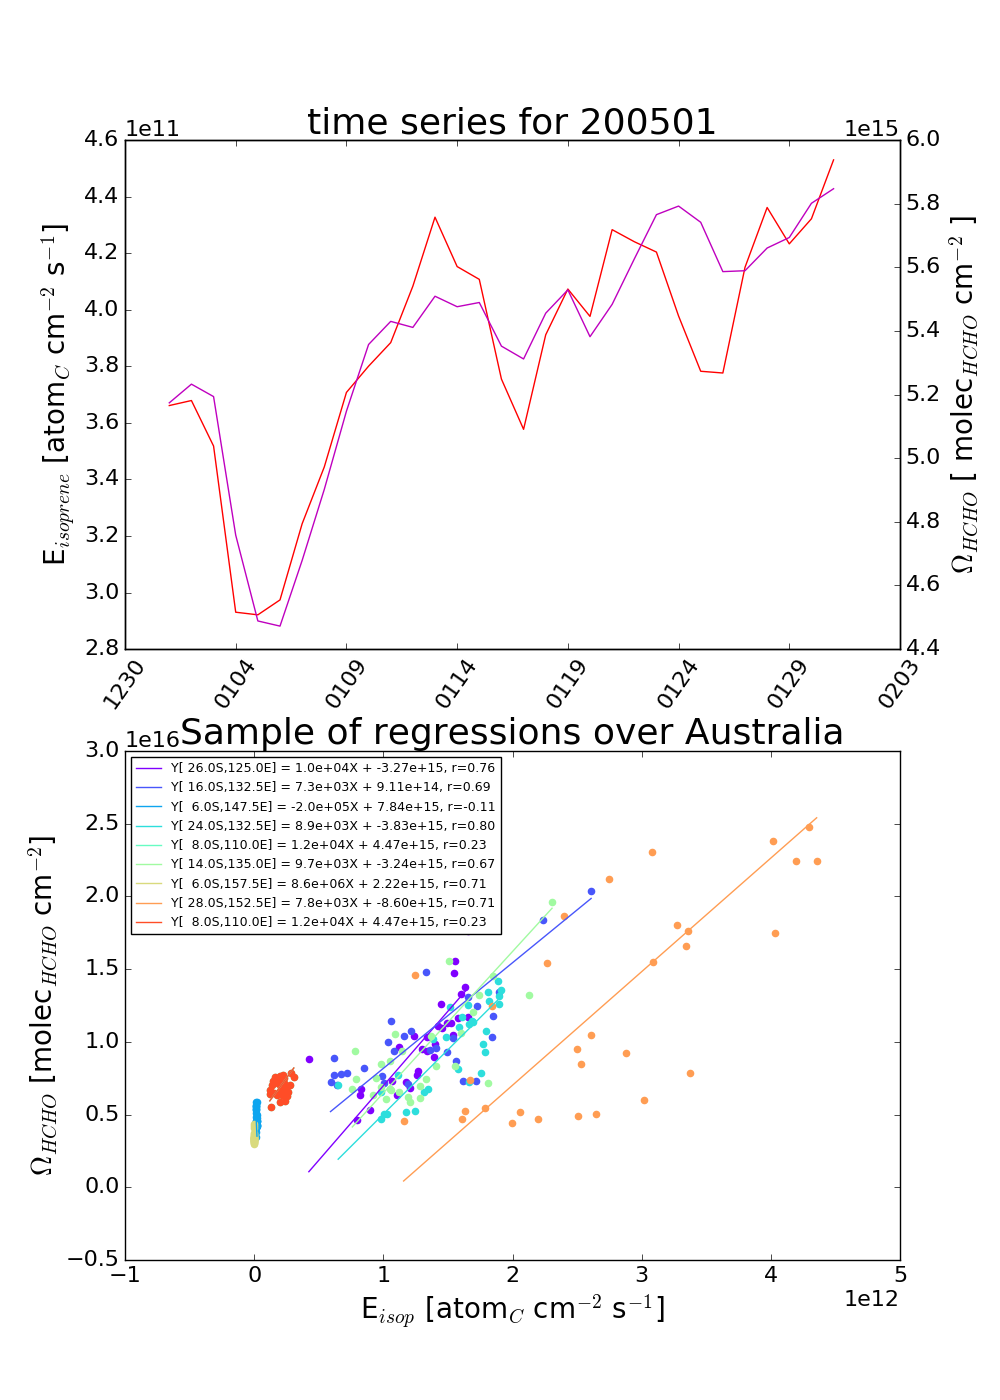
\includegraphics[width=\textwidth]{Figures/Isoprene/E_isop_vs_hcho_series_200501.png}
      \caption{%
        Top panel: isoprene emissions for January, 2005, shown in red, coplotted with tropospheric hcho columns, shown in magenta.
        Both series are daily averages over Australia.
        Bottom panel: (RMA) linear regressions from between emissions of isoprene and tropospheric hcho columns, sampled randomly from the 2$^{\circ}$ by 2.5$^{\circ}$ latitude longitude gridboxes over Australia for the month of January (2005).
      }
      \label{BioIsop:Calculation:fig_E_isop_vs_hcho_model_sample}
    \end{figure}
    
    %TODO: put this into results
    Using this modelled slope at 2$^{\circ}$ by 2.5$^{\circ}$ and applying it to equation \ref{BioIsop:Calculation:eqn_isop_yield} with B and $\Omega_{HCHO}$ calculated using OMI satellite measurements provides a new estimate of isoprene emissions.
    Figure \ref{BioIsop:Calculation:fig_E_isop_200501} shows the emissions calculated this way along with the Emissions output by GEOS-Chem averaged over January, 2005.
    \begin{figure}[!htbp]
      % Figure from Inversion.py -> check_against_MEGAN()
      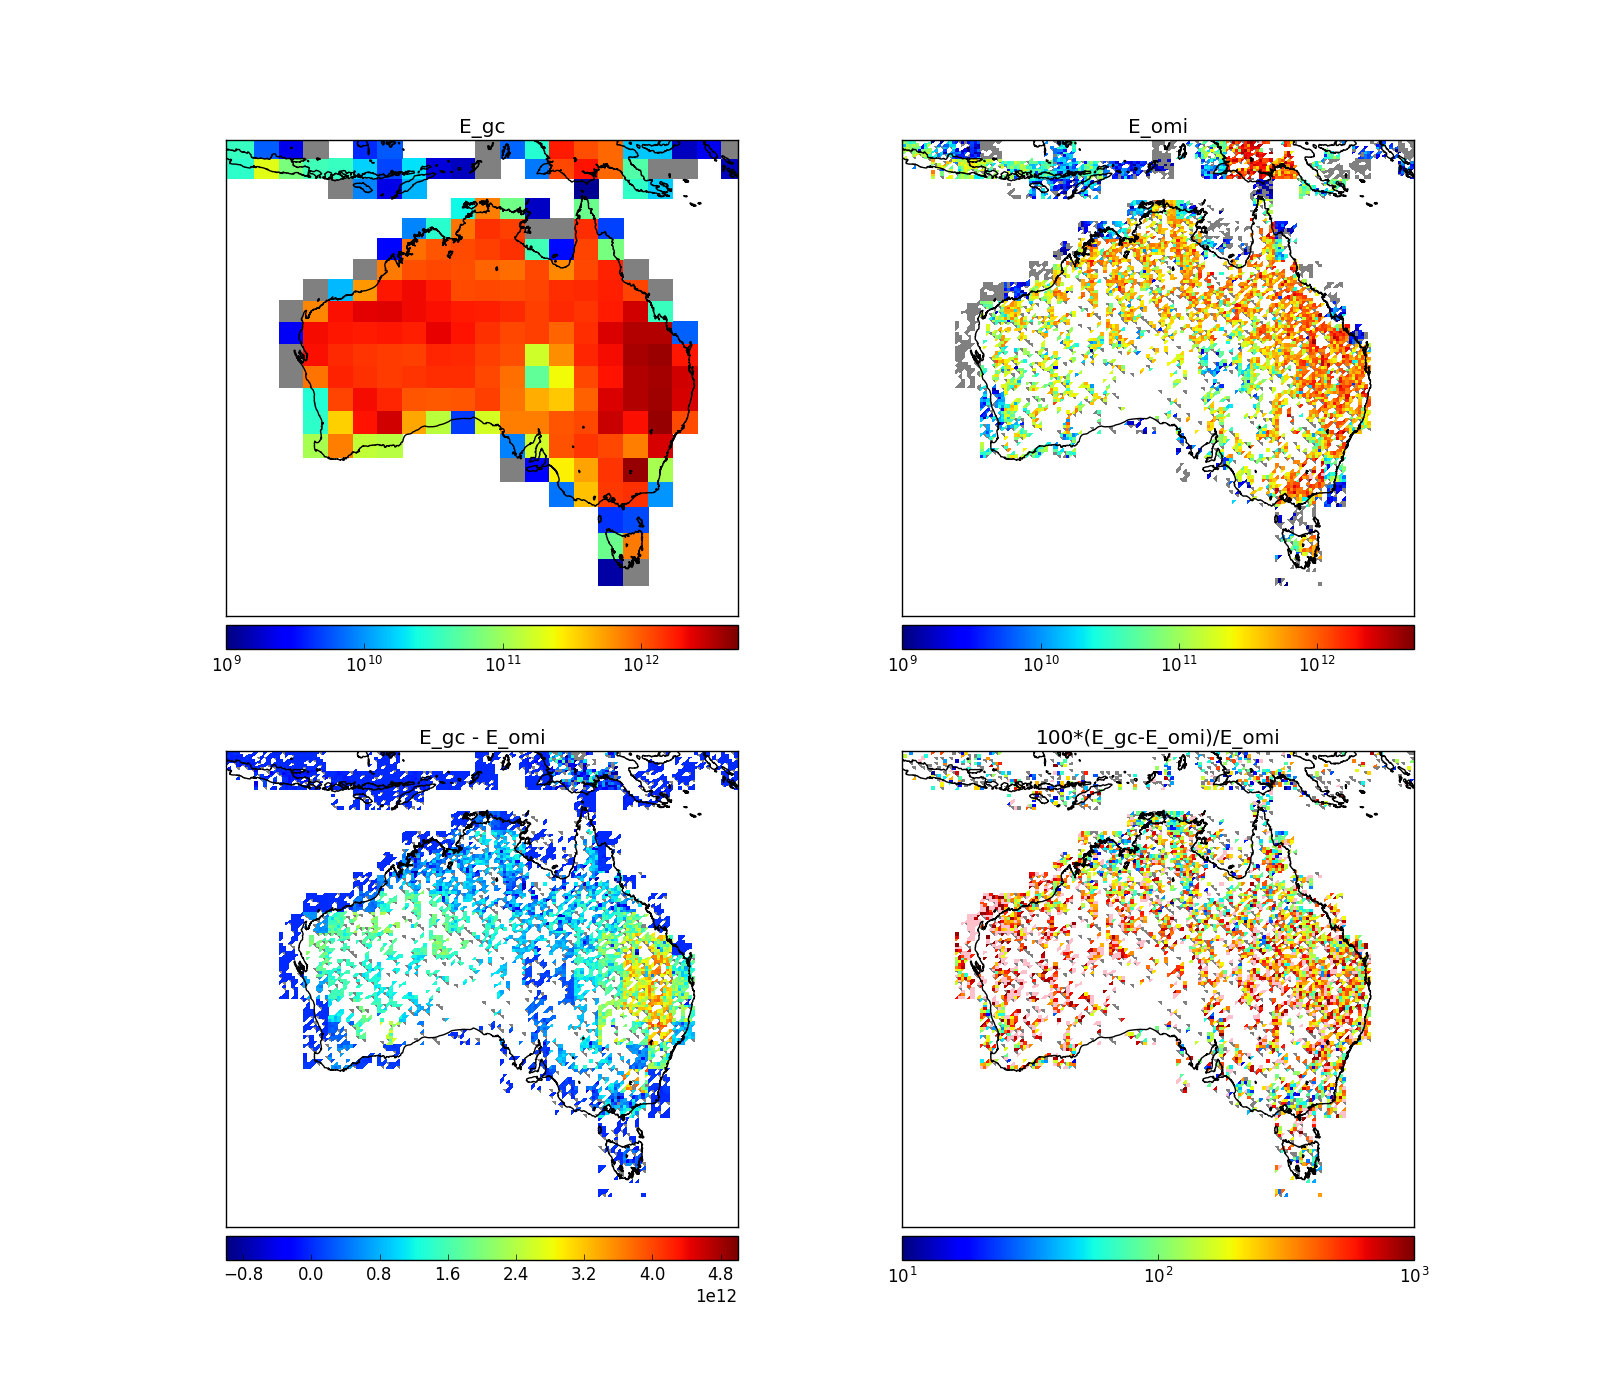
\includegraphics[width=\textwidth]{Figures/Isoprene/E_Comparison.png}
      \caption{%
        Top row is isoprene emissions for the month of January, in 2005, from GEOS-Chem and estimated from OMI respectively.
        Bottom row shows the absolute and relative differences between the two.
      }
      \label{BioIsop:Calculation:fig_E_isop_200501}
    \end{figure}
    
  
  \subsection{Accounting for smearing}
    \label{BioIsop:Method:Smearing}
    
    Accounting for transport of the precursors is important, especially in low NO$_X$ conditions in which isoprene has a longer lifetime (hours-days).
    When estimating emissions of isoprene using one of its products, it is often assumed that isoprene has a short lifetime, however when low NO$_X$ environments (which are prevalent in the Australian outback) this assumption can be wrong.
    Smearing is a measure of how much formaldehyde (the product) was created from isoprene (the precursor) emissions in a different grid box.
    Smearing has been measured in order to account for this uncertainty in various works \parencite[eg.][]{Martin2003,Palmer2003,Millet2006,Stavrakou2009,Marais2012,Barkley2013,Zhu2014,Wolfe2016,Surl2018}, often implementing the method designed in \textcite{Palmer2003}.
    One method to calculate the affects of smearing (performed in \textcite{Stavrakou2009}) involves an analysis of an adjoint CTM.
    A simpler method calculates smearing using two almost identical model runs, one of which has isoprene emissions halved.
    This allows determination of which gridboxes are disproportionately affected by emissions from non-local sources.
    Consider halving the isoprene emitted globally and rerunning the model, one would expect HCHO enhancement (above background levels) to be halved in isoprene emitting gridboxes.
    %\textcite{Marais2012} additionally use airborn isoprene, MVK $+$ MACR (isoprene oxidation products), and HCHO measurements to check smearing in Africa where there is a sharp gradient of isoprene emitting vegetation from north to south.
    
    Similarly to smearing sensitivity calculations in \textcite{Marais2012}, we run GEOS-Chem with isoprene emissions halved, then calculate $\hat{S} = \frac{\Delta \Omega_{HCHO}}{\Delta E_{isop}} $, where $\Delta$ represents the monthly mean departure over 1300-1400LT from default run values.
    If $\hat{S}$ is large, then you can infer sensitivity to non-local isoprene emissions.
    A relatively large change in $\Omega_{HCHO}$ (compared to local emissions) suggests that HCHO is being formed from non-local isoprene emissions.
    This is sensitive to how E$_{isop}$ is determined, figure \ref{BioIsop:Method:Smearing:fig_smearing_def_2005} shows smearing over two seasons with E$_{isop} =$ daily averaged isoprene emissions (left column) and midday (1300-1400~LT) emissions (right column). 
    Essentially the midday isoprene emissions are at the peak of their daily cycle (see figure TODO) which means the effect of smearing is relatively smaller during these hours.
    Figure TODO: shows the same figure with added markers showing when the threshold of 4000 \parencite[as in][]{Marais2012} affects at least one day within the season (pink diamonds) and where it removes all data for that gridbox (red x).
    
    \mypic{/Figures/OMI_link/Filters/smearing_definitions_2005.png}{Smearing ($\hat{S}$, see text) in summer (DJF, top row) and winter (JJA, bottom row) using averaged isoprene emissions daily (left column) and 1300-1400~LT (right column). Note that the scale changes between left and right columns.}{\label{BioIsop:Method:Smearing:fig_smearing_def_2005}}
    
    
    % Marais 2012 also look at average windspeed and best hcho-isop corelation when hcho is shifted by 0.5 degrees, don't think I can do that with 2.5 degree resolution
    % Marais compare smearing with model estimated yield " 
    
    
    Smearing can be dependent on local or regional weather patterns, as greater wind speeds will reduce the time any emitted compound stays within the local grid box.
    As such smearing sensitivity is both spatially and temporally diverse, shown in figure TODO: is a picture of the smearing sensitivity over Australia.
    Large smearing values can be seen near many coastlines as only a fraction of the grid squares actually emit isoprene, which makes transported isoprene relatively more important in these gridboxes.
    Once the smearing sensitive grid squares are filtered out, application of equation \ref{ch_isop:eqn:isop_yield} gives us an estimate of isoprene emissions across the nation.
    
    TODO: Plots of S hat showing worst smearing affected areas per season.
    
    TODO: Figure (TODO scatter plot of $\hat{S}$ vs $\Omega_{NO_2}$) shows how smearing is related to NO$_X$ over Australia.
    Figure (TODO same but binned by nox columns at about 0.1e15 width, over a longer time)
    
    \subsubsection{Smearing length scale}
    
      Horizontal transport complicates estimation of precursor emissions, as emitted compounds react beyond local gridboxes.
      The distance travelled (L) downwind (d) by a precursor (i) before becoming HCHO can be estimated using:
      \begin{equation*}
        L_{d,i} = \frac{U}{k_i - k_{HCHO}} \ln{ \left( \frac{k_i}{k_{HCHO}} \right) }
      \end{equation*}
      where U is wind-speed.
      \textcite{Palmer2003} further define a smearing length scale: L$_{s,i}$ as the distance downwind where a fraction (1 - $1/e$) of the precursor is completely transformed into HCHO.
      This equation uses the initial VOC column concentration ($[VOC]_0$) at the point of emission and mass balance equations as follows:
      \begin{equation}
      \frac{1}{k_{HCHO}-k_i} \left( k_{HCHO} \exp{ \left[ \frac{-k_i L_{s,i}}{U} \right]} -k_i \exp{ \left[ \frac{-k_{HCHO} L_{s,i}}{U} \right]} \right) = \frac{1}{e} 
      \end{equation}
      with limiting values L$_{s,i} \rightarrow U/k_i$ for $k_i << k_{HCHO}$, and L$_{s,i} \rightarrow U/k_{HCHO}$ for $k_{HCHO} << k_i$.
      Figure TODO: shows a rough estimate of isoprene smearing (L$_{isop}$) in Australia using wind speeds from TODO:, and reaction rates k$_{isop}$, k$_{HCHO}$ from GEOS-Chem.
      %TODO make this plot!
    
\section{Results}
  \label{BioIsop:Results}
  
  %TODO: Preliminary results shown at AGU - leading into other stuff
  
  
    \subsection{HCHO Products and yield}
    \label{BioIsop:Results:HCHOYield}
    Australian forests are strong emitters of both isoprene and monoterpenes, which go on to form various products including secondary organic aerosols, oxygenated VOCs (OVOCs), ozone, OH, and HO$_2$.
    This production occurs over several steps, yields are often classed into at least two categories.
    First generation HCHO yield refers to the amount of HCHO produced per unit isoprene consumed by initial oxidation, total yield (sometimes molar yield) refers to time dependent yield of HCHO over multiple oxidation stages \parencite{Wolfe2016}.
    \textcite{Wolfe2016} define prompt yield as the change in formaldehyde measurement per unit change in initial isoprene emissions.
    Some argue that isoprene emissions are overestimated, due to the fact that they are based on relatively few measurements of isoprene emission factors \parencite{Winters2009, FortemsCheiney2012} TODO: read and cite paper mentioned in Fortems.
    
    
    Isoprene production of HCHO depends on several factors, importantly NO$_X$ levels have a direct effect on the fate of VOCs in the atmosphere.
    At higher NO mixing ratios (at least a few hundred pptv), organic peroxy radicals (RO$_2$) react mostly with NO. 
    At low NO (less than 10's of pptv), reaction with HO$_2$, other RO$_2$, and isomerization dominate the fate of RO$_2$.
    In low NO$_X$ environments, reported HCHO yields from isoprene are from XtoY\%, while in high NO$_X$ environments this value is XtoY\% TODO: these values from table.
    For monoterpenes the yields are around X, Y\% for low, high NO$_X$ respectively.
    Emissions and yields for various species including some terpenes can be seen in table \ref{BioIsop:Method:tab_VOCAusYields}.
    \textcite{Wolfe2016} determine that going from NO$_X = 0.1$ to $2.0$ ppbv triples the prompt yield of HCHO, from 0.3 to 0.9 ppbv ppbv$^{-1}$ due to isoprene, while the background HCHO doubles.
    They determine prompt yield as the change in HCHO per change in ISOP$_0$, using $[ISOP]_0=[ISOP]\exp(k_1[\mathrm{OH}]t)$; where $k_1$ is first order loss rate.
    This effectively relates HCHO abundance with isoprene emission strength.
    %TODO:and finish Wolfe2016 discussion paper for yields
    
    NO$_2$ measured by OMNO2d gives us a daily mid-day measurement which we can compare to output from GEOS-Chem to determine how well the model does at simulating NO$_2$.
    This is also done in \textcite{Travis2016}, as a way to examine model bias in ozone (potentially due to NO$_2$ bias) over the USA.
    
    Conversions between HCHO per unit C yield and molar \% yield from species X given by the equation $ Y_{molar \%} = 100 \times C_X \times Y_{HCHO per unit C} $, where $C_X$ is how many Carbon are within species X (5 for isoprene, 10 for monoterpenes, etc...).
    For instance a 200\% molar yield of HCHO from isoprene implies 1 Mole of C$_5$H$_8$ becomes 2 Mole HCHO which is a 0.4 HCHO per unit C yield.
    
    TODO: Fill out this table
    \begin{table} \begin{threeparttable}
        \caption{HCHO yields from various species averaged over Australia during Summer.}
        \begin{tabular}{ | c  c  c  c  c | }
          \toprule
          \textbf{Species}   & \textbf{Emissions$^a$}& \textbf{Lifetime$^b$}& \textbf{HCHO Yield$^c$} & \textbf{HCHO production$^d$\%}
          \\                 & (Tg C per month)      &                      & (per C reacted)         &         \\
          \midrule
          Isoprene           & Y                     & n minutes            & 0.x                     & 10       \\
          $\alpha$-Pinene    & Y                     & n minutes            & 0.x                     & 10       \\
          $\beta$-Pinene     & Y                     & n minutes            & 0.x                     & 10       \\
          HCHO               & Y                     & n minutes            & 1.0                     & 10       \\
          \bottomrule
        \end{tabular}
        \begin{tablenotes} 
          \item a: Calculated using GEOS-Chem emissions over Australia in January 2005.
          \item b:  
          \item c: 
          \item d: Production determined by dividing emission*yield by the sum of all VOC emissions*yields. 
        \end{tablenotes}
        \label{BioIsop:Method:tab_VOCAusYields}
      \end{threeparttable} \end{table}
      
      % yields from Atkinsen2003
      %isoprene
      %0.63 0.10 Tuazon and Atkinson (1990a)
      %0.57 0.06 Miyoshi et al. (1994)
      % a-pinene
      %0.23 0.09 Noziere et al. (1999a)
      %0.19 0.05 Orlando et al. (2000)
      % b-pinene
      %0.54 0.05 Hatakeyama et al. (1991)
      %0.45 0.08 Orlando et al. (2000)
      
      Yields table looking at literature provided yields of HCHO.
      % molar HCHO yield per unit carbon equal to HCHO molar percent yield(per carbon)? or some conversion?
      % TODO: ask steve about ppbv ppbv^-1 ??
      
      \begin{table} \begin{threeparttable}
          \caption{ HCHO yields from various species, and lifetime against oxidation by OH. }
          \begin{tabular}{  l  l  l  l  l  }
            \toprule
            Species    & HCHO Yield    & Life vs OH   & NO$_X$ background & Source   \\
            & (molar \% )   &              &                   &          \\
            \midrule 
            Isoprene	& 315$\pm$50      &            & High          & a        \\ 
            & 285$\pm$30      &            & High          & a        \\ 
            & 225             & 35 min     & High          & b        \\ % Done
            & 150             &            & Low           & b        \\ % Done
            & 150             &            & Low           & d        \\
            & 450             &            & High          & d        \\
            & 235             &            & 1~ppbv        & e        \\
            & 150             &            & 0.1~ppbv      & e        \\
            $\alpha$-Pinene & 28$\pm$3        &        & Low                & c        \\ 
            & X$\pm$3         &        & X                  & d        \\ 
            & 230$\pm$90      &        & High        & a        \\ 
            & 190$\pm$50      &        & High        & a        \\ 
            & 19              & 1 hour &              & b        \\ % Done
            & 210             &        & 1~ppbv        & e        \\
            & 70              &        & 0.1~ppbv      & e        \\
            $\beta$-Pinene  & 65$\pm$6        &        & Low           & c      \\ 
            & X$\pm$3         &        & X             & d      \\ 
            & 540$\pm$50      &        & High          & a     \\ 
            & 450$\pm$80      &        & High          & a      \\ 
            & 45              & 40 min &              & b      \\ % Done
            Methane 	      & 100             & 1 year  &             & b     \\ 
            Ethane          & 180             & 10 days &             & b     \\ 
            Propane         & 60              & 2 days  &             & b     \\ 
            Methylbutanol   & .13(per C)    & 1 hour  &             & b     \\ 
            HCHO            & 100             & 2 hour  &             & b     \\ 
            Acetone         & .67(per C)      & 10 days &             & b     \\ 
            Methanol        & 100             & 2 days  &             & b     \\ %Done
            \bottomrule
          \end{tabular}
          \begin{tablenotes} % \item makes new lines
            \item a \textcite{AtkinsonArey2003}: Table 2, Yield from Isoprene reaction with OH, two values are from two referenced papers therein.
            \item b \textcite{Palmer2003}: lifetimes assume [OH] is 1e15 mol cm$^{-3}$.
            \item c \parencite{Lee2006}: Calculated through change in concentration of parent and product linear least squares regression.
            Estimates assume 20$^\circ$~C conditions.
            \item d \textcite{Wolfe2016}: ``prompt yield'': change in HCHO per change in ISOP$_0$.
            $[ISOP]_0=[ISOP]\exp(k_1[\mathrm{OH}]t)$; where $k_1$ is first order loss rate.
            Effectively relates HCHO abundance with isoprene emission strength
            \item e \textcite{Dufour2009}: One-day yields from oxidation modelled by CHIMERE, using MCM reference scheme.
            \item f Calculated using PTR-MS and iWAS on SENEX campaign data.
          \end{tablenotes}
          \label{BioIsop:Method:tab_VOCLiteratureYields}
        \end{threeparttable} \end{table}
        
        Looking at Australian emissions from running GEOS-Chem and using yields provided by XYZ (TODO other table), we see that Australia may be more or less likely to be affected by both NO$_X$ and pollution and high wind speeds TODO: this comparison sentence would be good to tie up tables and be copied to conclusions.  
        
  \subsection{Emissions comparisons}
    \label{BioIsop:Results:Emissions}
  
    Some global numbers (TODO: where do I throw these?)
    \textcite{Guenther2012} Estimate global biogenic isoprene emissions at roughly 535\tgpyr, using MEGAN.
    \textcite{Sindelarova2014} Estimate around 594\tgpyr using MEGAN with MACC, showing isoprene as 69.2\% of the total BVOC emissions, with monoterpenes at 10.9\tgpyr (10.9\%).
    They show 41\tgpyr decrease in Australia when introducing soil moisture parameterisation.
    When comparing the GEOS-Chem (which runs MEGAN) emissions to those calculated using our top-down inversion, we see a decrease over TODO: locations and seasons.
    TODO: table or figure showing summary of isoprene emissions changes over the whole of our time domain.
    
    Most recently a \textcite{Bauwens2016} estimated isoprene emissions with this technique using the IMAGESv2 global CTM.
    They calculate emissions which create the closest match between model and satellite vertical columns, and compare these postiori data with the apriori (satellite data) and independent data sets.
    They found TODO: what they found and how this analysis differs from my own.
    (TODO: simple outline of what they did and how my focus is different, this paper will also need to be summarised in the LitReview)
    
    Satellite measured HCHO has been found to be biased low in several studies \textcite[eg.][]{Zhu2016,DeSmedt2015,Barkley2013}.
    These papers use in-situ data to scale up the satellite HCHO columns for their areas of interest, however Australia lacks sufficient HCHO measurements to do this.
    In these papers bias is seen as high as 40\%, which we use as our upper bound.
    We scaling up the satellite columns by 40\% and use this as an upper bound on the uncertainty due to satellite bias.
    The 'Scaled Satellite' column refers to the calculations when using the 40\% scaled up OMI HCHO columns. %TODO: make table, add that column.
    
    Figure todo shows the emissions over Australia averaged within January 2005.
    This figure shows estimates from MEGAN (top), and top down estimates using OMHCHO $\Omega$s (row 1: OMI), $\Omega$ recalculated using GEOS-Chem shape factors (row 2: GC), and using the code from Paul Palmer's group (row 3: PP).
    Column 2 is emissions without applying anthropogenic or pyrogenic filters, Column 3 is calculated at the lower resolution of 2x2.5\degr.
    
    Figure todo shows emissions over time from a single grid square, estimated by MEGAN (black) and the three top-down estimates, using 2x2.5\degr horizontal resolution.
    
    Figure todo shows emissions over Australia calculated using the OMI top down estimate (column 1) and MEGAN (column 2). 
    The black line is the average and over Australia, while the red line is the average for within the red rectangle. 
    Grey shading shows the 25th to 75th percentile for all of Australia.
    
  \subsection{Comparison with in-situ measurements}
    
    TODO: % TODO: campaign analysis compared to GEOS-Chem
    Analyse comparison of gridbox with campaigns of measurements
    
    One set of data from the Daintree rainforest in Queensland exists (TODO: summary from P. Nelson).
    Although the data set lies outside our run times, as it was measured in TODO(runtime), we compare against the seasonal average of our GEOS-Chem output for the matching months (TODO: name the months).
    This is done for both GEOS-Chem output and our recalculated isoprene emissions.
    When compared against GEOS-Chem output we see TODO.
    When compared against recalculated emissions we see TODO.
    
    TODO: Figure showing campaign data against model and recalculated emissions over region for averaged months and eventually different resolutions.

 \section{Affects of emissions on chemistry}
 
   \subsection{HCHO levels}
     
     %As is done in \textcite{Emmerson2016}, 
     We examine the affect of decreased isoprene emissions on the correlation between modelled and satellite based HCHO columns.
     Figure TODO: shows the regressions between GEOS-Chem tropospheric column amounts of HCHO and satellite columns for two runs of GEOS-Chem: a) using standard MEGAN emissions, b) using our updated emissions.
     We interpolated or something (TODO) the emissions over Australia into the inventories used by GEOS-Chem which reduced the emissions by X\% per year (over Australia).
     The resulting simulation output shows that HCHO was reduced by X\%, although if we boost monoterpenes by X\% where the isoprene emissions were lowered then 
     
   \subsection{Ozone levels}
   
     TODO: compare ozone after changing isoprene emissions in GEOS-Chem

\section{Uncertainty}
\label{BioIsop:Uncertainty}

  There are several factors which need to be considered when looking at the uncertainty in emissions estimates.
  Things with their own inherent uncertainty include the modelled a-priori, modelled relationship between HCHO and isoprene, and satellite measurements. 
  Important factors which need to be analysed for confidence in results include the steady state assumptions, filtering techniques for fire and human influences, and the regression model for determining the isoprene to HCHO yield.
  
  Uncertainty in satellite HCHO, along with top down emissions estimates $E_{isop}$ is listed in table \ref{Model:Uncertainty:tab_uncertainties}.
  %\textcite{Millet2006, Palmer2006} both examine OMI HCHO columns over North America and determine overall uncertainty to be 40\%, with most of this coming from cloud interference.
  \begin{table}\begin{threeparttable}
    \caption{Uncertainties in literature and here.}
    \begin{tabular}{ l | c  c  l } 
      \toprule
      product & uncertainty & location & notes \\
      \midrule
      satellite HCHO & 40\% & North America & (a) mostly due to cloud interference \\
       & X\% & where & (b) \\
      top-down $E_{isop}$ & Y\% & where & (c) \\
       & X\% & Australia & accumulated uncertainty in calculation \\
       & X\% & Australia & range found when scaling satellite HCHO \\
      \bottomrule
    \end{tabular}
    \begin{tablenotes} 
      \item a: \textcite{Millet2006,Palmer2006}
      \item b: 
    \end{tablenotes}
    \label{Model:Uncertainty:tab_uncertainties}
  \end{threeparttable}\end{table}
  
  \subsection{Model Uncertainty}
    \label{Model:Uncertainty:Model}
    
    
    Model uncertainty is difficult to accurately ascertain, generally an analysis of the model compared to in-situ measurements is performed, however there are few of these measurements over Australia.
    Here GEOS-Chem output is compared against the campaign datasets with the caveat that in-situ and point measurements are quite different to modelled (large) area averages.
    
    
    Uncertainty in modelled yield is estimated somehow (TODO:).
    Prior works use flight campaigns and in-situ data to verify HCHO columns in various locations (TODO: redo cite list from lit review).
    Figures X to D TODO: make figures comparing campaigns to model HCHO
    Yield calculations are performed at low resolution (2\degr x 2.5\degr) which may lead to overestimation \parencite{Yu2016}.
    TODO: how do I check this?
    
  % Subsection?
  \subsection{Satellite Uncertainty}
    \label{BioIsop:Uncertianty:Satellite}
    
    There are three main sources of error in the satellite HCHO columns:
    \begin{description}
      \item[a] Fitting error from the OMI retrieval.
      \item[b] Uncertainty in AMF calculations.
      \item[c] Uncertainty of HCHO background.
    \end{description}
    a) is available in the OMI product and reduced through spatial and temporal averaging.
    Taking the eight day gridded average with horizontal resolution of 0.25 by 0.3125 degrees (latitude by longitude) typically reduces uncertainty by a factor of 1.5 to 4.
    b) is determined through an analysis of GEOS-Chem output, validated against the total column of HCHO at Wollongong using FTIR measurements from the (TODO: Nicholas Jones roof HCHO citation here).
    \textcite{Palmer2006} calculate the error in AMF through combining estimates of error in the UV albedo database ($\sim 8$\%), model error based on in-situ measurements, cloud error  ($20-30$\%) \parencite{Martin2003}, and aerosol errors ($<20$\%), totalling AMF error of around $\sim 30$\%.
    It is worth noting here that independent error estimates are added in quadrature, which means total error equals the root of the sum of the independent errors each squared ($e_{Total}=\sqrt{\Sigma_i e_i^2}$).
    TODO:Paul palmer calculation and combination for overall Satellite VC uncertainty per pixel and gridded.
    TODO: Millet2008?
    c) is also determined through a study of GEOS-Chem output, in relation to in-situ measurements.
    TODO: calculate this uncertainty.
    Compare this error estimate with that of \textcite{Curci2010}, where the error in b) and c) are respectively found to be 30\% and 15\% based on their analysis of CHIMERE.
    \textcite{Millet2008} also examine this uncertainty and determine an overall uncertainty ($1\sigma$) of $25-27\%$ in HCHO vertical columns with calculated AMFs where cloud fraction $< 0.2$.
    
    
    Two simple methods of looking at overall uncertainty from satellite measurements are performed here.
    \begin{enumerate}
      \item using the variance over the remote pacific ocean to provide relative uncertainty globally \parencite[e.g.][]{DeSmedt2012}
      \item scaling up HCHO columns by 40\% as an upper bound on satellite uncertainty
    \end{enumerate}
    Analysing variance over the remote pacific gives a quick measure of uncertainty if we assume HCHO levels within the region are stable.
    This region should be relatively invariant throughout any month so each month the standard deviation of the midday total column HCHO amounts from 15\degr S to 15\degr N, and 180\degr W to 120\degr W.
    Other literature has found satellite HCHO columns to be up to 40\% too low, so scaling them up 40\% is another way of quickly analysing how sensitive our calculations are to the satellite HCHO columns.
    
    TODO: Calculate remote pacific variance (also bin by latitudes) and plot over time. 
    
    
    Provided with the OMI product is the measurement of uncertainty in each pixel, calculated by SAO from the backscattered solar radiation fit \parencite{Abad2015,Abad2016}.
    Uncertainty introduced through AMF calculation needs to be additionally determined to give a representation of the confidence in vertical column amounts.
    BIRA use another method, and calculate the standard deviation of HCHO over the remote pacific ocean as the uncertainty \parencite{DeSmedt2012, DeSmedt2015}.
    In the remote pacific, it can be assumed that HCHO variations are weak, with concentrations remaining steady in the short term ($\sim 1$ month).
    This means the standard deviation over this region can be used as a proxy for determination of the instrument error.
    
    
    TODO: uncertainty calculation on remote pacific OMI.
    
    OMI is scaled up by up to 40\% in several papers (cite) we consider HCHO scaled by 1 and 1.4 to be boundaries for modelled yield.
    In effect this scales the top down emissions estimate by 1.4.
    Plot TODO shows the affect on $E_{isop}$ if we scale satellite HCHO up by 40\%, with the solid line being the original isoprene emissions and the dashed line showing the 40\% increase. TODO: Make sure this is true and make the plots.
    
  \subsection{Fire Filtering}
    
    %Look at emissions estimates with and without the fire filter applied
    Figure \ref{BioIsop:Uncertainty:Fire:fig_emiss_without_fire_filter} shows emissions estimates for January 2005, using three different HCHO columns as the basis: the original OMI satellite HCHO columns ($\Omega$), those with AMF recalculated using a new apriori ($\Omega_{GC}$), and those with AMFs recalculated using PP code ($\Omega_{PP}$).
    The first row shows emissions estimates calculated as shown in \ref{BioIsop:Methods}, while the second row runs the same calculations without applying any fire or smoke filter.
    The Third row is the absolute difference between them: fire filtered minus standard emissions.
    
    \mypic{Figures/OMI_link/Emiss/FireFilter200501.png}
    {Emissions estimates using OMI satellite columns (column 1) recalculated with updated shape factor (column 2) and scattering weights (column 3). Turning off the fire and smoke filters gives emissions in row 2, while the difference between row 1 and row 2 is shown in row 3.}
    {\label{BioIsop:Uncertainty:Fire:fig_emiss_without_fire_filter}}
    
    % TODO: Emissions Averages and differences over the year with and without a fire filter 
  
  \subsection{MEGAN}

    One of the important parameters in Australia is the soil moisture activity factor($\gamma_{SM}$), which can have large regional effects on the isoprene emissions \parencite{Sindelarova2014,Bauwens2016}.
    Generally if soil moisture is too low, isoprene emissions stop \parencite{Pegoraro2004,Niinemets2010}, however in many Australian regions the plants may be more adapted to lower moisture levels. (TODO: Find cites for this - talk from K Emerson at Stanley indicated this)
    GEOS-Chem runs MEGANv2.1, which has three possible states for isoprene emissions based on the soil moisture ($\theta$):
    \begin{align*}
    \gamma_\mathrm{SM} & = 1 && \theta > \theta_1 \\
    \gamma_\mathrm{SM} & = (\theta-\theta_w)/\Delta\theta_1  && \theta_w < \theta < \theta_1 \\
    \gamma_\mathrm{SM} & = 0 && \theta < \theta_w \\
    \end{align*}
    where $\theta_w$ is the wilting point, and $\theta_1$ determines when plants are near the wilting point.
    The wilting point is set by a land based database from \textcite{Chen2001}, while $\theta_1$ is set globally based on \textcite{Pegoraro2004}.
    Potentially importantly, these moisture states are disabled in GEOS-Chem V10.01, which is partly because accurate maps of soil moisture are not available.

\section{Conclusions}
  \label{BioIsop:Conclusions}
  
% Extras for potential paper output 
%  
%  \authorcontribution{}
%  \competinginterests{The authors declare that they have no conflict of interest.}%
%  \textit{Data availability.} All GEOS-Chem model output is available from the authors upon request.
%  %\disclaimer{disclaimer}
%  \begin{acknowledgements}
%    This research is supported by an Australian Government Research Training Program (RTP) Scholarship.
%  \end{acknowledgements}
  